\section{Extrapolations to higher luminosity}
\label{sec:extrapolations}

Future runs of the LHC expect to deliver significantly higher instantaneous luminosity than current operations. To cope with these harsher data-taking conditions, upgrades to the muon spectrometer are planned. In Long Shutdown 2 which is scheduled to start in 2018, the current endcap small wheels will be replaced by the New Small Wheels equipped with small Thin Gap Chambers (sTGC) and MicroMegas (MM) detectors. In Long Shutdown 3, which is scheduled to start near 2022, an additional round of upgrades is now being planned as the LHC will enter its high-luminosity phase, the HL-LHC.

% the MDT electronics are being considered for replacement, and additional coverage for the barrel muon trigger system is under consideration.

A crucial ingredient in the planning of these upgrades is the hit rate of incident particles the detectors are expected to receive. This section presents an expected rate in the hottest regions of the MS as extrapolated from data-taking in 2015. This extrapolation does not address potential changes in the ATLAS shielding or the beam pipe, or the particle sensitivity of future detector technologies, both of which can have a large effect and must be characterized with simulation. The hottest regions of the MS in 2015 data are the innermost regions of the endcap inner small wheel (CSC L, CSC S, MDT EIL1, MDT EIS1) and endcap middle big wheel (EML1, EMS1).

The hit rates presented in Section~\ref{sec:hitrates} of the note include all hits reported by the detectors, including those from electronic noise. The contribution from electronic noise is detector-dependent, hence the inclusive hit rate may be less useful for projecting to future LHC conditions because new detectors (sTGC, MM) will be deployed in the NSW. The projections are split into two parts to address this. First, the inclusive hit rates are projected and can be considered an upper-bound of the future rates. Second, hit rates with hit quality criteria cuts (\textit{ADC cuts}) are projected, which remove a large fraction of electronic noise while maintaining good efficiency for hits from incident particles. This is a more accurate reflection of the conditions for future MS detectors, though an unfolding to particle fluxes is still not attempted. Here, the criteria for suppressing electronic noise are at least 50 ADC counts for an MDT tube and at least 100 ADC counts for the highest-ADC strip in a CSC cluster. The MDT (CSC) quality criteria is assumed to be fully (78.9\%) efficient for incident charged particles.

The predictions are performed by considering the hit rates in 2015 data-taking as a function of the instantaneous luminosity, fitting the linear dependence, and extrapolating to higher luminosity. These rates are shown in Section~\ref{sec:hitrates} with linear fits overlaid, for the inclusive hit rates.

The parameters of the linear fit depend on the number of filled bunches in the LHC, as expected. The maximum number of filled bunches in 2015 is 2232 bunches, whereas Run 3 of the LHC is expected to fill at most 2808 bunches, and the HL-LHC is expected to fill at most 3564 bunches. To extrapolate to more filled bunches, the fitted slopes are considered for 2015 runs with as few as 447 filled bunches and as many as 2232 bunches, and the dependency is extracted by fitting this spectrum to a first-order inverse power law, as shown in Figure~\ref{fig:extrapolations-slope-vs-bunches-raw} with vertical lines at 2808 and 3564 filled bunches. The fitted slopes are the same as reported in Figures~\ref{fig:hitrates-vs-lumi-csc-raw}, \ref{fig:hitrates-vs-lumi-mdt-ei1-raw}, and \ref{fig:hitrates-vs-lumi-mdt-em1-raw}. The same procedure is followed for the projected hit rates with ADC cuts.

\begin{figure}
  \begin{center}
    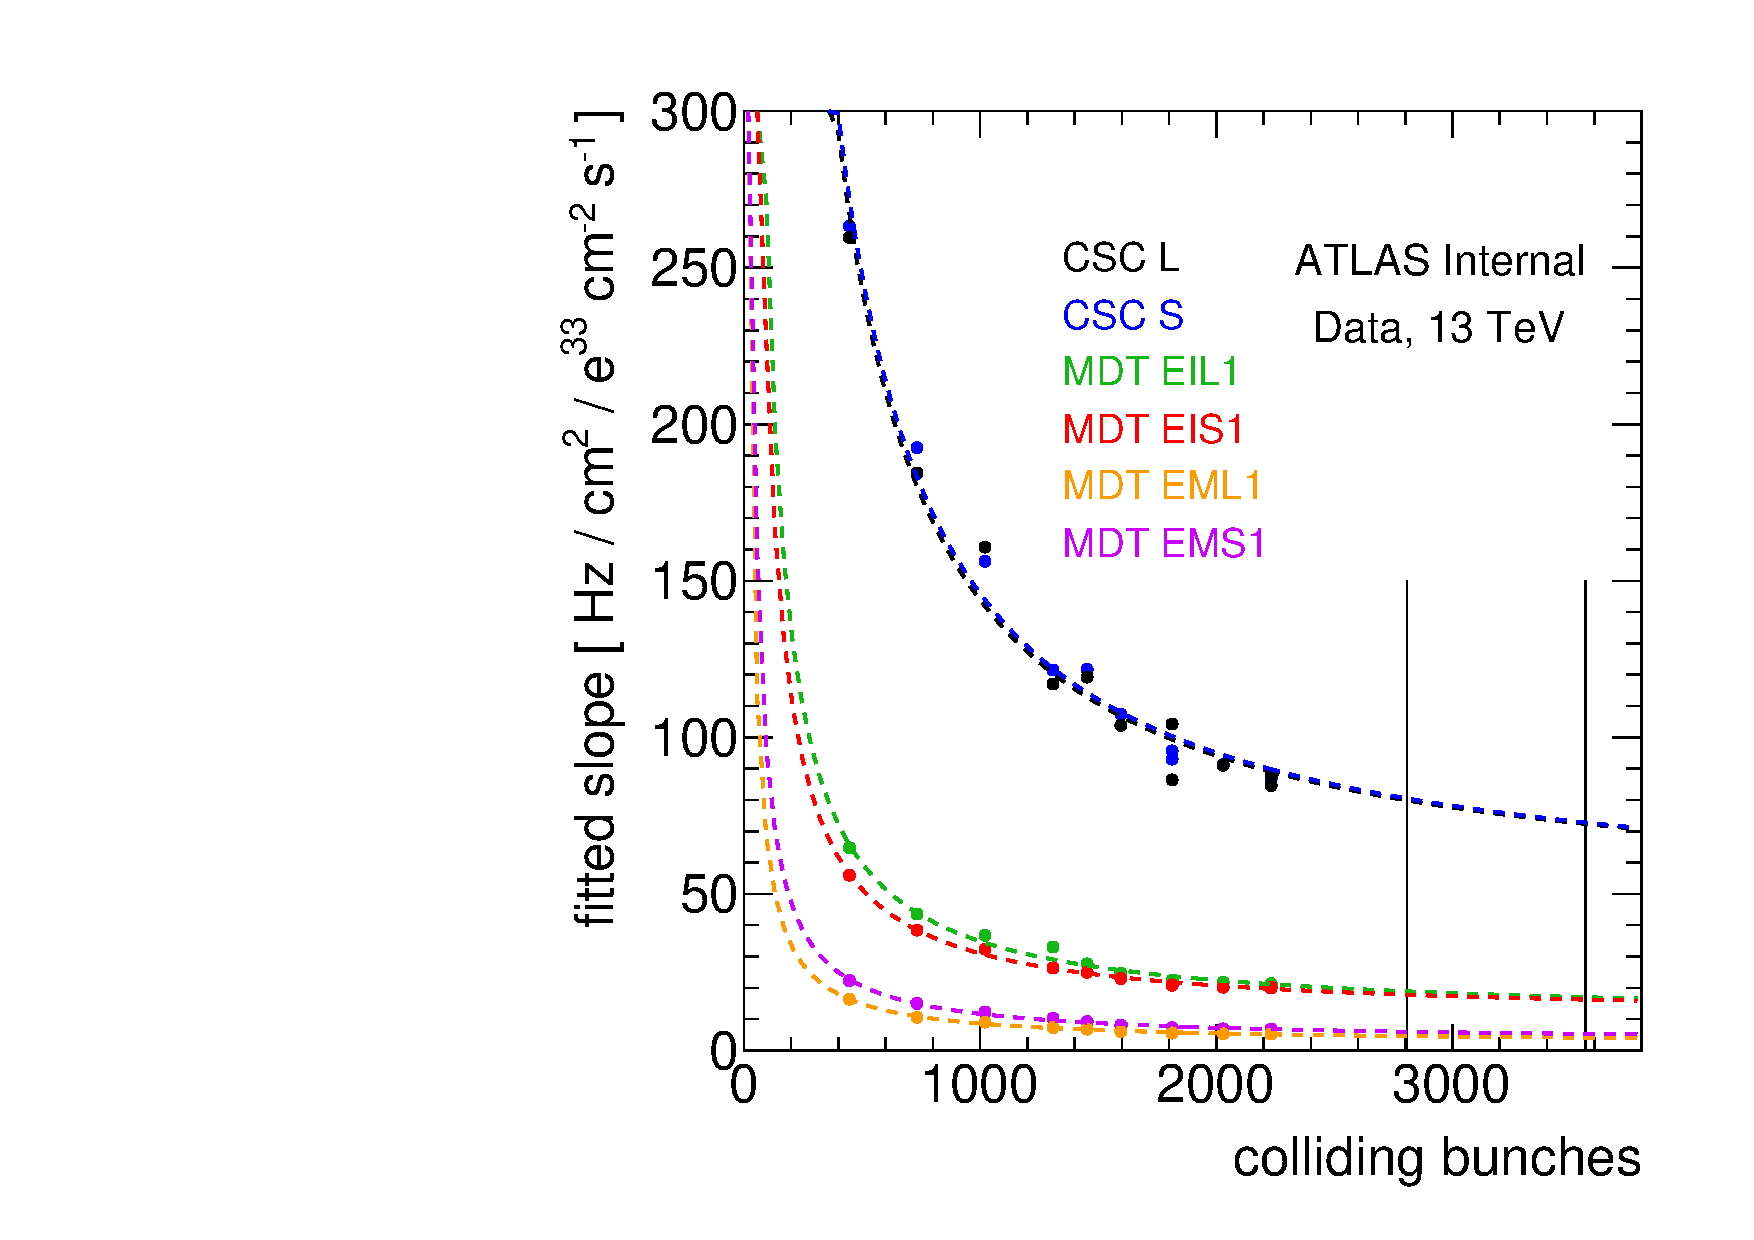
\includegraphics[width=0.45\textwidth]{./figures/slope_vs_bunches_raw_lin.pdf}
    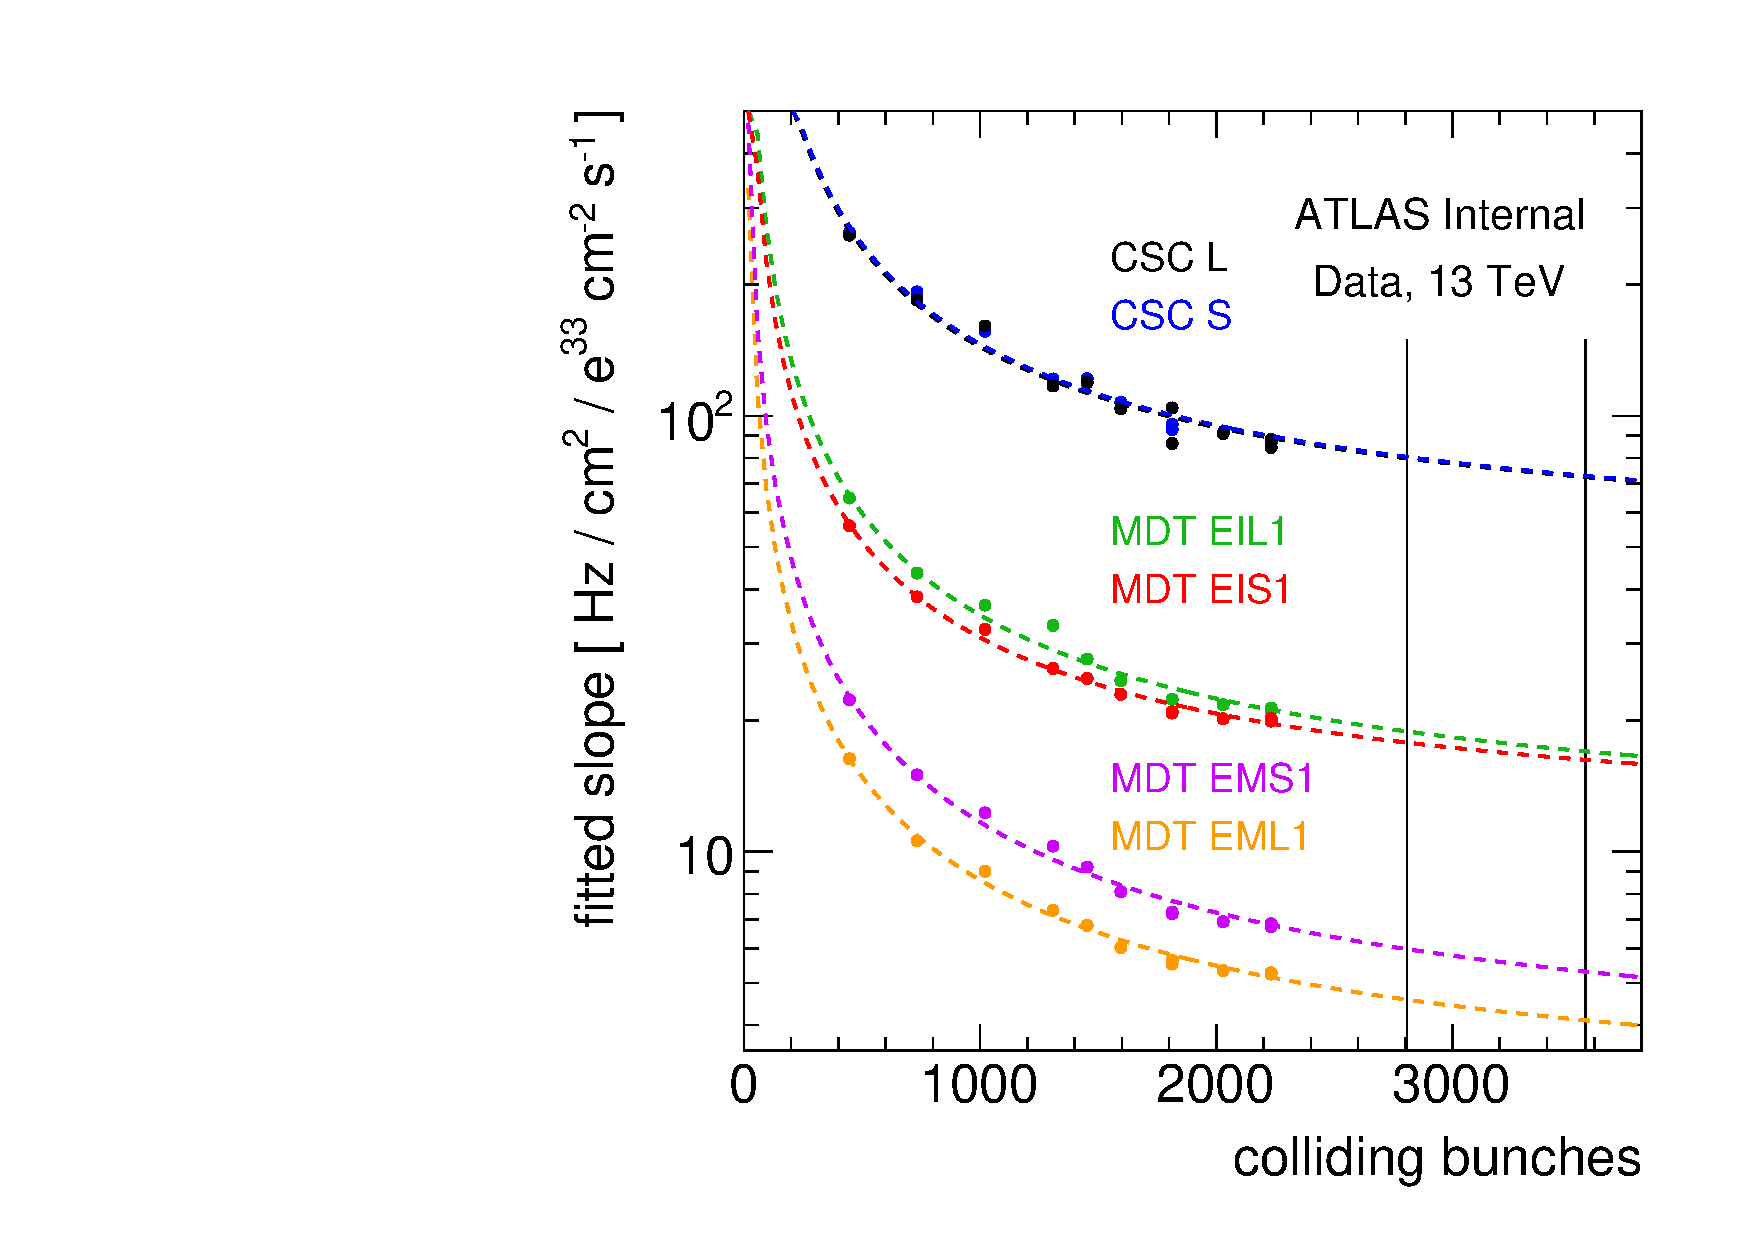
\includegraphics[width=0.45\textwidth]{./figures/slope_vs_bunches_raw_log.pdf}
    \caption{The fitted slope for inclusive hit rates as a function of the number of colliding bunches for various runs in the hottest MDT and CSC chambers, shown with linear (left) and logarithmic (right) scale. The spectra are fitted to $A + B/x$, where $x$ is the number of bunches.}
    \label{fig:extrapolations-slope-vs-bunches-raw}
  \end{center}
\end{figure}

This fit gives parameters for the linear dependence of hit rate on instantaneous luminosity at more filled bunches than was reached in 2015. The projected inclusive hit rates for the hottest chambers of the MS are shown in Figure~\ref{fig:extrapolations-hitrates-raw}. The large (L) and small (S) sectors of a given detector region have similar projected hit rates.

\begin{figure}
  \begin{center}
    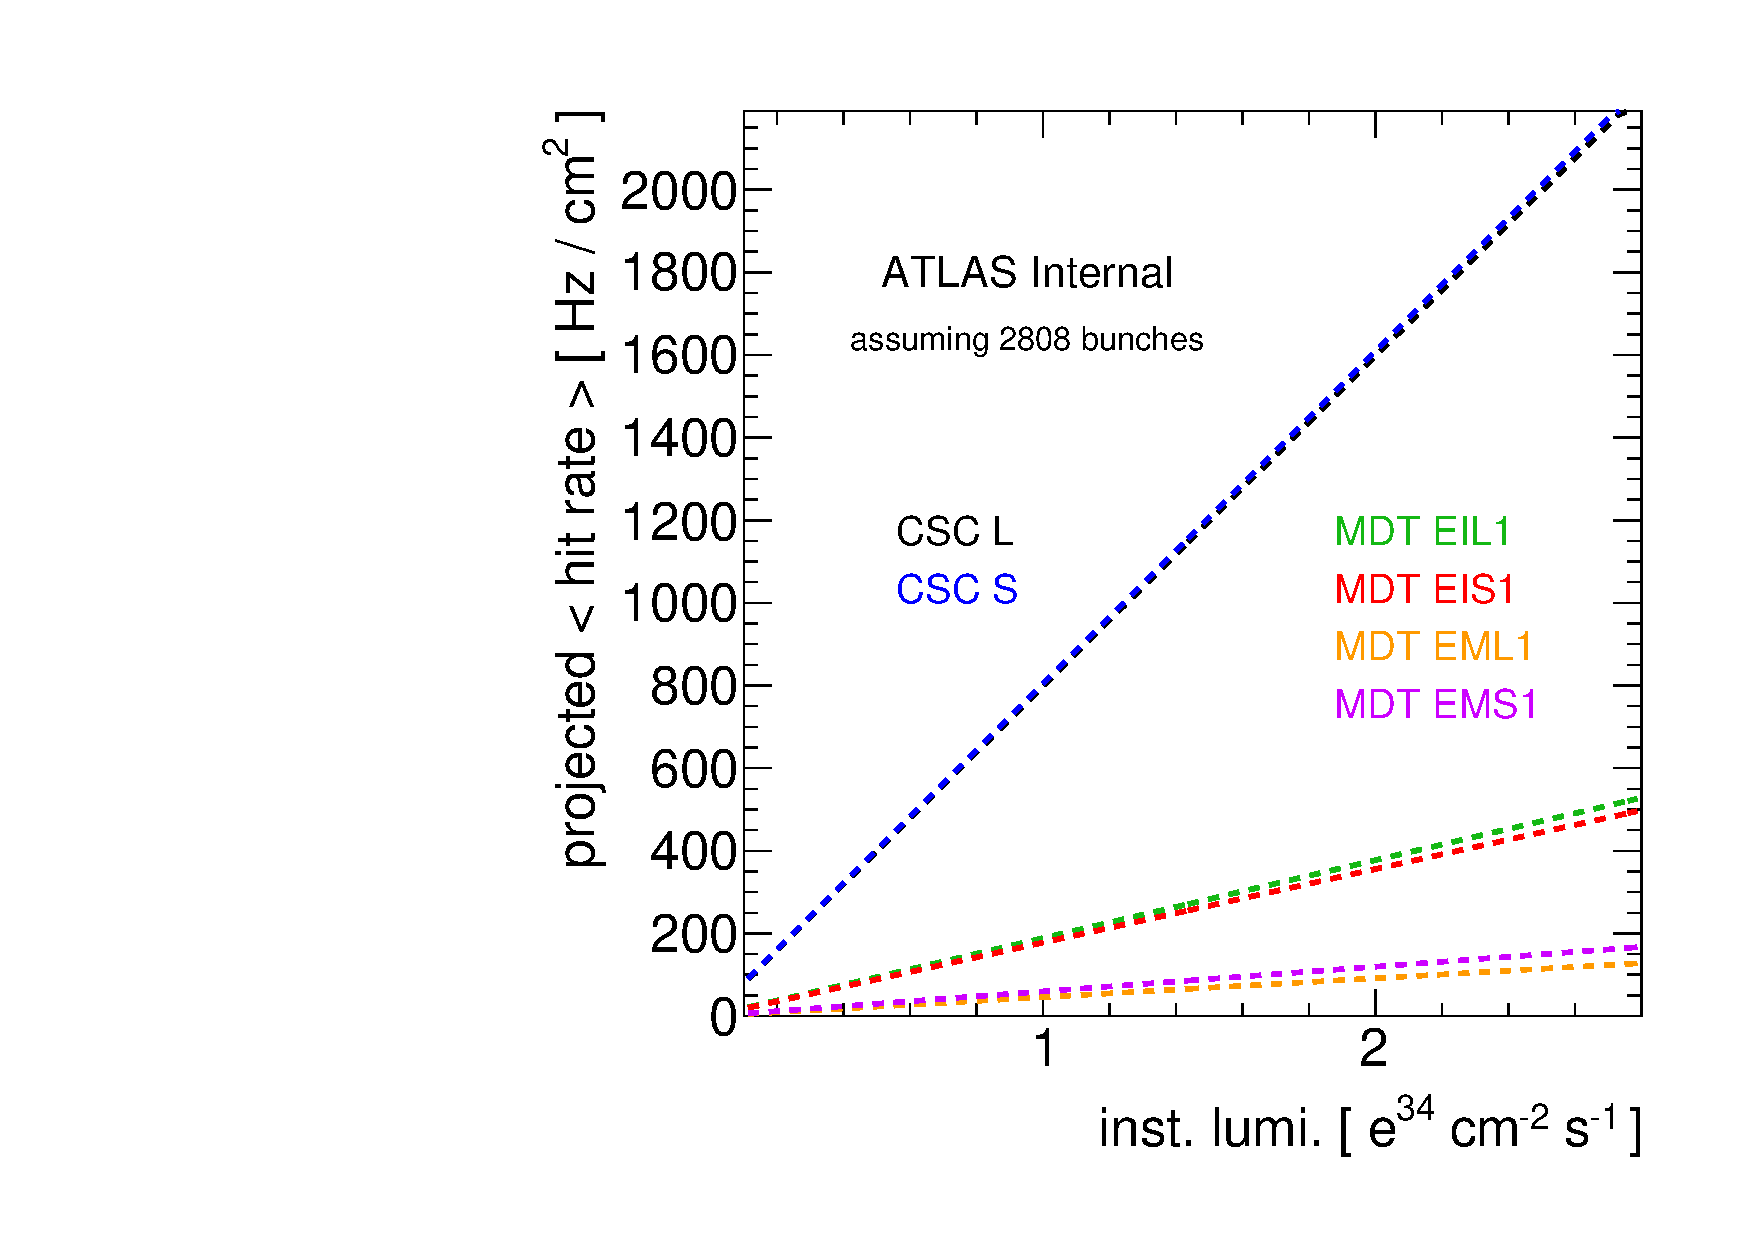
\includegraphics[width=0.45\textwidth]{./figures/extrapolate_vs_lumi_raw_2808.pdf}
    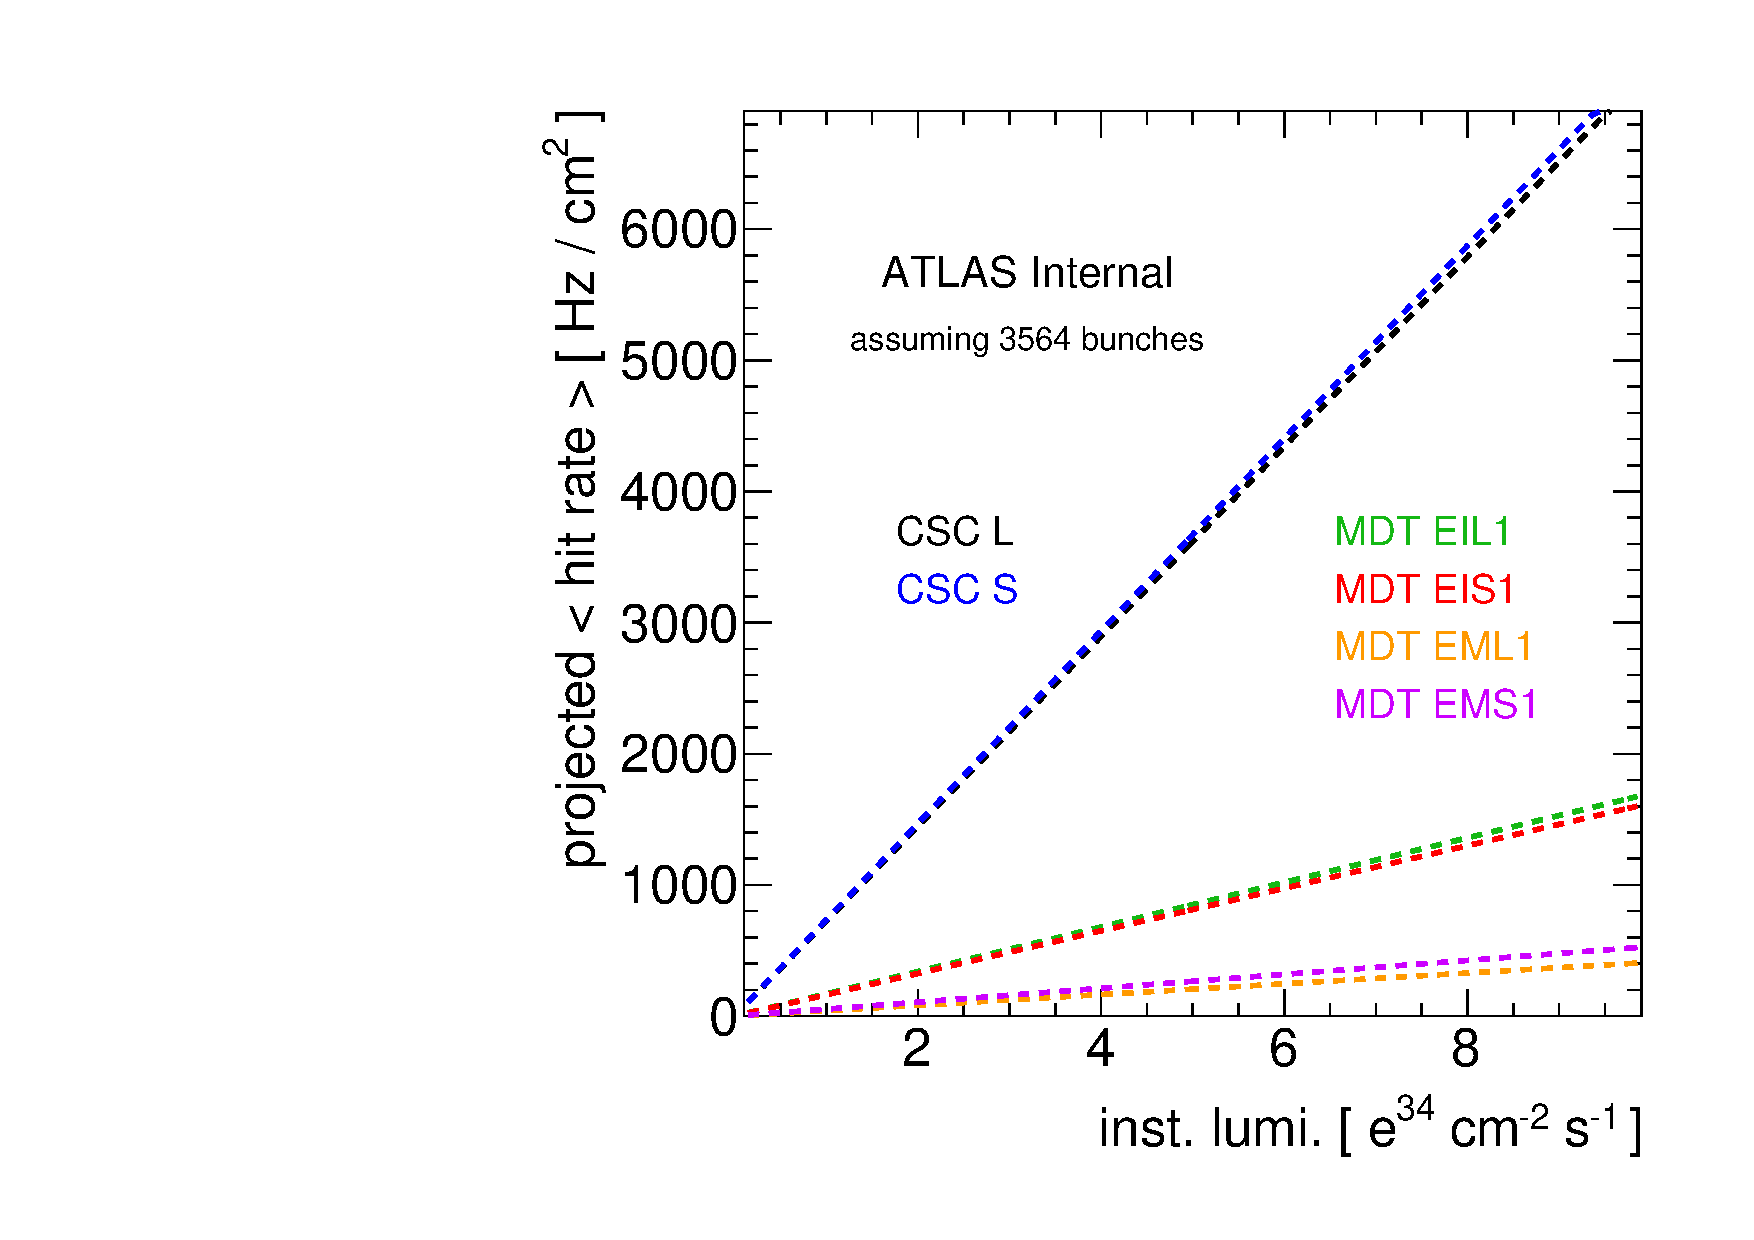
\includegraphics[width=0.45\textwidth]{./figures/extrapolate_vs_lumi_raw_3564.pdf}
    \caption{Projected inclusive hit rates in the MS as a function of instantaneous luminosity, assuming 2808 (left) and 3564 (right) filled bunches in the LHC. The CSC and MDT EI regions are overlaid.}
    \label{fig:extrapolations-hitrates-raw}
  \end{center}
\end{figure}

The projected average hit rates at Run 3 and HL-LHC conditions are shown in Table~\ref{tab:extrapolations-hitrates}, both inclusively and with ADC cuts. The instantaneous luminosity is assumed to be $2\times10^{34}$ in Run 3 and $7\times10^{34}$ at the HL-LHC. 

\newcommand*{\hspfou}{\hspace*{0.4cm}}

\begin{table}
  \begin{center}
    \renewcommand{\arraystretch}{1.4}
    \begin{tabular}{c||c|c||c|c}
      \multicolumn{1}{c}{}   & \multicolumn{4}{c}{\rate} \\
      \multicolumn{1}{c}{}   & \multicolumn{2}{c}{inclusive}                  & \multicolumn{2}{c}{with ADC cut} \\
      \hspsix Region \hspsix & \hspsix Run 3 \hspsix & \hspfou HL-LHC \hspfou & \hspsix Run 3 \hspsix & \hspfou HL-LHC \hspfou \\
      \hline\hline
      CSC L                  & 1598                  &  5065                  & 1093                  & 3338 \\
      CSC S                  & 1609                  &  5095                  & 1094                  & 3342 \\
      \hline
      MDT EIL1               &  377                  &  1189                  &  321                  & 1007 \\
      MDT EIS1               &  356                  &  1137                  &  304                  &  968 \\
      \hline
      MDT EML1               &   92                  &   287                  &   77                  &  241 \\
      MDT EMS1               &  120                  &   372                  &  100                  &  309 \\
      \hline\hline
      NSW, hottest           & 3560                  & 11200                  & 2420                  & 7390 \\
    \end{tabular}
    \caption{Projected hit rates at Run 3 and HL-LHC conditions in the hottest regions of the MS, both inclusively and with ADC cuts. Run 3 conditions assume $\mathcal{L}=2\times10^{34}$ and 2808 filled bunches in the LHC. HL-LHC conditions assume $\mathcal{L}=7\times10^{34}$ and 3564 filled bunches.}
    \label{tab:extrapolations-hitrates}
  \end{center}
\end{table}

The CSC hit rate in 2015 data-taking closest to the beampipe is at most $\sim\!2.2$ times larger than the average hit rate of the chamber, as discussed in Section~\ref{sec:hitrates}. This implies the hottest region of the small wheel at HL-LHC conditions will have a hit rate of 11.2 $\text{kHz} / \text{cm}^2$ when hits in 2015 data-taking are considered inclusively. The corresponding hit rate is 7.4 $\text{kHz} / \text{cm}^2$ when hits are considered with ADC cuts. These projections assume no changes in the ATLAS shielding or beam pipe.

The extrapolations here are generally consistent with previous extrapolations using the Run 1 dataset \cite{CERN-LHCC-2013-006,ATL-COM-MUON-2013-003,ATL-COM-MUON-2013-011}. The regions of the CSC closest to the beam pipe project to have a rate which is within the benchmark of 15 $\text{kHz} / \text{cm}^2$ considered in the NSW technical design report. Projections of the MDT hit rates are about 20\% lower than the Run 1 projections, which is expected from simulation, given the updates to the ATLAS beam pipe and shielding during Long Shutdown 1 \cite{ATL-COM-MUON-2014-027}.
